\documentclass[10pt,journal,final,letterpaper,twocolumn]{IEEEtran}
%\documentclass{ssdbm}
\usepackage{wrapfig,subfigure,setspace,verbatim,cite,url,graphicx,float}
\usepackage{algorithmic,amsfonts,amssymb,amsmath,calc,calrsfs,cleveref}
\usepackage[justification=centering]{caption}
%\usepackage{fixltx2e}

\restylefloat{table}

% This was from the NEW paper
%----------------------------------------------------------
\RequirePackage{fix-cm}

\DeclareMathOperator{\var}{var}
\newcounter{qcounter}

%\smartqed  % flush right qed marks, e.g. at end of proof
%----------------------------------------------------------

\newtheorem{theorem}{Theorem}
\newtheorem{lemma}{Lemma}
\newtheorem{definition}{Definition}
\newtheorem{remark}{Remark}

\newcommand{\SEC}[1] {Section \ref{#1}}
\newcommand{\Eq}[1] {Equation \ref{#1}}
\newcommand{\eq}[1] {Eq. (\ref{#1})}

% correct bad hyphenation here
\hyphenation{op-tical net-works semi-conduc-tor}


\begin{document}

% paper title
\title{Parallelization of Push-based System for Molecular Simulation Data Analysis with GPU}

% author names and IEEE memberships
% note positions of commas and nonbreaking spaces ( ~ ) LaTeX will not break
% a structure at a ~ so this keeps an author's name from being broken across
% two lines.
% use \thanks{} to gain access to the first footnote area
% a separate \thanks must be used for each paragraph as LaTeX2e's \thanks
% was not built to handle multiple paragraphs

\author{Iliiazbek~Akhmedov, Yi-Cheng~Tu~$\dagger$, Vladimir Grupcev, Joseph Fogarty, Sagar Pandit % <-this % stops a space

%\thanks{* These authors contributed equally to this work.}
\thanks{$\dagger$ Author to whom all correspondence should be sent.}
\thanks{Iliiazbek Akhmedov, Vladimir Grupcev, and Yi-Cheng Tu are with the Department of Computer Science and Engineering, University of South Florida, 4202 E. Fowler Ave., ENB 118, Tampa, FL 33620, U.S.A. Emails:
akhmedovi@mail.usf.edu, ytu@cse.usf.edu}
\thanks{Joseph Fogarty and Sagar Pandit are with the Department of Physics,
University of South Florida, 4202 E. Fowler Ave., ISA 2019, Tampa,
FL 33620, U.S.A. Emails: jcfogart@mail.usf.edu, pandit@usf.edu} }

%\pubid{0000--0000/00\$00.00~\copyright~2002 IEEE}

% use only for invited papers
%\specialpapernotice{(Invited Paper)}

% make the title area
\maketitle

\begin{abstract}

Modern simulation systems generate big amount of data, which consequently has to be analyzed in a timely fashion. Traditional database management systems follow principle of pulling the needed data, processing it, and then returning the results. This approach is then optimized by means of caching, storing in different structures, or doing some sacrifices on precision of the results to make it faster. When it comes to the point of doing various queries that require analysis  of the whole data,  this design has the following disadvantages: considerable overhead on random I/O while reading from the simulation output files and low throughput of the data that consequently results in long latency, and, if there was any indexing to optimize selections, overhead of storing those becomes too big, too. 

There is a new approach to this problem presented in the previous paper -- Push-based System for Molecular Simulation Data Analysis for processing network of queries proposed in the previous paper and its primary steps are: i) it uses traditional scan-based I/O framework to load the data from files to the main memory and then ii) the data is pushed through a network of queries which consequently filter the data and collect all the needed information which increases efficiency and data throughput. It has a considerable advantage in analysis of molecular simulation data, because it normally involves all the data sets to be processed by the queries.

In this paper, we propose improved version of Push-based System for Molecular Simulation Data Analysis. Its major difference with the previous design is usage of GPU for the actual processing part of the data flow. Using the same scan-based I/O framework the data is pushed through the network of queries which are processed by GPU, and due to the nature of science simulation data, this gives a big advantage for processing it faster and easier. In the old approach there were some custom data structures such as quad-tree for calculation of histograms to make the processing faster and those involved loss of data and some expectations from the data nature, too. In the new approach due to high performance of GPU processing and its nature, custom data structures were not even needed much though it didn't bear any loss in precision and performance.

\end{abstract}

\begin{IEEEkeywords}
Push-based system, molecular simulation, scientific databases,
spatial distance histogram, GPU, parallel processing, CUDA.
\end{IEEEkeywords}
%\vspace{-5mm}

%%%%%%%%%%%%%%%%%%%%%%%%%%%%%%%%%%%%%%%%%%%

\section{Introduction}\label{sc:intro}

In various sciences simulation systems take big place and often times they may be the clue for results. One of such sciences, which is primarily related to this paper, is physics. In this case, from computer engineering point of view, simulations have the following flow:

\vspace{5mm}

{\small
\begin{enumerate}
	\item initial physical properties are given to simulation software as arguments which are interpreted and provided in a language defined by the simulation software
	\item then it runs for given amount of time that can generally last from milliseconds to months or even more
	\item finally, the file generated during the simulation is analyzed to extract useful information
\end{enumerate}
}
\vspace{3mm}
The purpose of this paper is primarily focused on the third step, which basically involves the entire simulation data to be processed by the analysis software.

Big data processing is becoming one of the key issues with the amount of data being generated by modern systems. Eventually, this data is required to be processed on the fly, thus, analysis software should be able to handle massive data in a very short period of time. When working with huge volume of data, there are non-trivial issues arise. For example, it can take days and weeks to analyze big enough data sets, because the data cannot be simply loaded into memory, since it can get up to terabytes, thus, it has extra overhead because of widely used random access disk I/O framework to read from disk chunks by chunks. Besides it, analysis of the data can get even more complicated, since going through certain parts of the data once would not be enough, which leads to low throughput and efficiency of loaded data. One such example, the data analysis approach has polynomial complexity just for reading the data in order to come up with result, and since the data can't simply be saved in memory, it raises the overhead of disk I/O, too. Pull-based architectures in data processing engines are inefficient, since having a set of specific queries, in order to compute them all, it is needed to fetch data, filter it, and apply needed formulas. It is inefficient, since for every query the same chunk of data needs to be pulled into the memory at least the number of queries times or more in case of more complex queries.

As it has already been mentioned in the previous paper \cite{mainPaper}, one of the modern issues of analyzing massive data on the fly is social networks. .
"In order for a system to be able to perform analytical examination of the data produced in such streaming media, the system should have the capability of fast data access. The reason, the millions of data records(tweets) produced
every second. Moreover, these tweets may have
different geographical origin, introducing different languages and
forms and often times containing unsolicited messages, errors,
malicious content, etc. Therefore, some low level data uniformity
and cleaning on top of the data access and management issues should
be considered and possibly incorporated in the process of analytical
investigation in order to achieve relevant result. "\cite{mainPaper, nature_bigdata08,nature_bigdata12,science_social10,jcs_twitter11}

The primary focus and problem in this paper is scientific data analysis. Particles simulation is one of the most popular methods of analyzing certain chemical reactions, physical processes, or other behavior of different materials.
Molecular simulations (Molecular Dynamics) are applied in different fields and represent a method of analyzing physical movements of particles, atoms, and molecules in a fixed space with a given period of time, apparently with a possibility of giving initial state for each item that is involved in the process and can affect the system. This system is an N-body simulation. The number of atoms in simulations vary in hundred of thousands, particularly, we may observe two simulation systems of a collagen fiber structure and dipalmitoylphosphatidylcholine (DPPC) bi-layer lipid system consisting of 890,000 and 402,400 atoms respectively on Figure \ref{fg:collagen_dipal}. Simulation data represents number of records of physical properties such as mass, charge, velocity, coordinates, and forces for each item aggregated as frames, where each frame represents a snapshot of time, placed with a fixed time interval which may also vary depending on the simulation itself and simulation precision requirement. "Quantities measured during the simulations are analyzed to test the theoretical
model~\cite{Frenkel:api01,Landau:cup05}. In short, the MS is proven
and powerful tool for understanding the inner-workings of a
biological system, by supplying a model description of the
biophysical and biochemical processes that are being unfold at a
nanoscopic scale." \cite{mainPaper}

Scientist gives the properties to simulation software (for example, Gromacs), runs the simulations, and finally get the output file. The output file must then be analyzed to produce certain results which may help him come up with certain consensus on original theoretical model that resulted in the molecular simulation system\cite{Frenkel:api01}. Gromacs is simulation software tool that helps scientist to run the actual simulation. It is a molecular dynamics package primarily designed for biomolecular systems such as proteins and lipids. \cite{Gromacs-online}. Besides the fact that it helps to generate the output files for the simulations, apparently it also helps to analyze the data itself, but the original problem is that it is not as optimized as it can be in order to analyze the data. Gromacs follows approach of pull-based design, which means that for any given query (e.g. total mass or total charge, which are very similar type of 1-body queries without sophisticated selection) it will pull data separately and generate addition overhead wasting disk read I/O in order to come up with the result just for a single query. As it has been proposed in the previous paper, in order to remedy such issues, the push-based design does exactly the opposite, where instead of loading the data on demand for each query, the queries are batched into a network, then the entire dataset is loaded chunk by chunk pushing it through the network which has its internal relationships and dependencies amonth the queries. In this case, since scientific simulation data is run once with specific physical properties, it is never modified, thus, on continuation, it will only append, which means that the processing can also be run on appended frames. \cite{mainPaper}
This type of approach has already been revised by other systems \cite {DataPath,Volcano,Qpipe} as of reusing loaded data through queries produced \cite {Candea,PredictablePerformance,CooperativeScans}.

In this paper, we are incorporating parallelization into the processing part of the proposed design by means of CUDA programming language for GPU. Since storage of the simulation data is very expensive, it might come to the point of analyzing the data on the fly (meaning running the simulation and analyzing it at the same time in a streaming manner), which leads to a problem of optimizing the processing part of the design proposed in the previous paper, because time spent on generating data should be tried to conceal the time spent on the processing part by means of overlapping or simply running it in a quick manner.

\begin{figure}
 \centerline{ 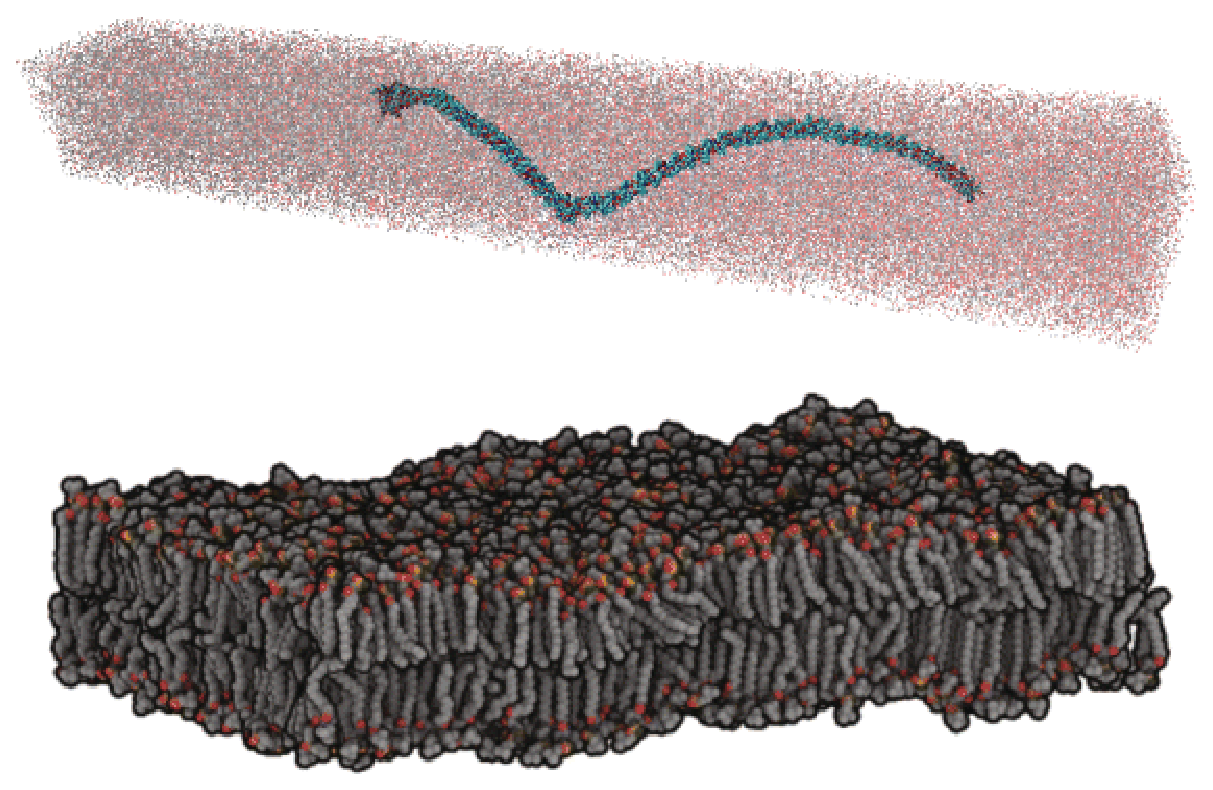
\includegraphics[width=1\columnwidth]{images/sample_snapshot_of_simulation.eps} }
 \caption{ Snapshots of two MS systems: a collagen fiber structure with 890,000 atoms (top) and a dipalmitoylphosphatidylcholine (DPPC) bi-layer lipid system with 402,400 atoms (bottom) \cite{mainArticle}}
 \label{fg:collagen_dipal}
\end{figure}

\subsection{Problem Statement}
Simulation software systems, in general, follow the same methodology of running and storing simulation data. The simulation software system examples are: Gromacs \cite{GROMACS4}, VMD\cite{VMD}, MDAnalysis~\cite{MDAnalysis}, Wordom~\cite{wordom}, MD-TRACKS~\cite{MDtracks}, SimulaidOne~\cite{Simulaid}, Charmm~\cite{CHARMM}. In the type of simulations brought up as examples above, the flow of the data is the following. Once the simulation is run, the output files are contained as trajectory files with descriptors (they contain information about space dimensions, number of atoms and frames, etc.) that can be easily transposed into simple flat files containing the physical properties atom by atom, frame by frame, which are consequently read and processed by the proposed push-based system. Since we have certain amount of queries needed to be run on given simulation data, generating high I/O traffic followed by design of pull-based system is not considerable. The approach proposed in the previous paper is very good in terms of performance in comparison with the original pull-based system\cite{mainPaper}. The problem is still that some of the queries processed by those means are still improvable, especially taking into consideration the fact that in the used previous works for calculation of 2-body functions, which take the biggest time for processing~\cite{ytu:icde09, EDBT12}, we might have some error bounds, which might be unacceptable for certain simulation analysis where sacrifice on loss of data is unbearable. Besides it, although we might have huge performance boost on specific data structure as density map, we still have certain expectation from data nature (such as its uniformity), thus, it makes sense to have desire to simplify the processing and still having pure computation based on any values, considering that the queries should be available to be pre-programmed by user in a separate module of the code.


\begin{figure}
 \centerline{ 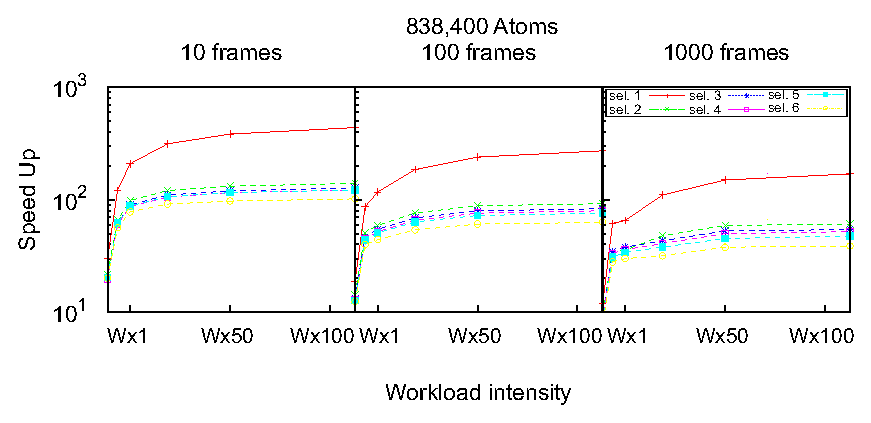
\includegraphics[width=1\columnwidth]{images/speedup838K-pomalo-za-4.eps} }
 \caption{ Speed up over different levels of atom selection for 838,400 atoms \cite{mainPaper}}
 \label{fg:sample_estimation_old_paper}
\end{figure}

\subsection{Our approach with improvement}

Reading the data from files is a huge overhead, thus, speedup of push-based system in general is significant over pull-based system in our given case. 
It's been demonstrated in the previous paper with different amount of atoms, frames, and workloads. Since we have to load the data every time there is a different query versus push-based system loads a chunk of data once, it is quite noticeable how the framework contributes to efficiency of analysis of simulation data. You can observe some estimation samples in Figure \ref{fg:sample_estimation_old_paper}. Even though the memory loading and pushing steps are the key features of the proposed design, nevertheless, having general knowledge about the network of queries, in this paper, we will try to focus on optimizing the actual execution of them.

Some of the queries may be very slow due to their nature on a sequential type of computation,  especially, 2-body functions. Since the nature of the data that comes with simulation is basically physical properties of atoms, there is a lot of computation that involves independent primitive mathematical operations, which makes it a perfect problem for parallelism.

Although the original idea of push-based system for molecular simulation data analysis was focused on optimizing throughput and usage of loaded data, there were some extra approaches specifically for 2-body functions. For example, Density Map for Spacial Distance Histogram was used in order to avoid additional memory allocation and latency reduction with proven error bounds. SDH is a quite intensive and computational problem, especially with increasing amount of atoms. 

We believe that having this nature of computational problems, the proposed GPU improved version of push-based system will significantly change in terms of performance by incorporating parallelism with CUDA.

%%%%%%%%%%%%%%%%%%%%%%%%%%%%%%%%%%%
%%%%%%%%%%%%%%%%%%%%%%%%%%%%%%%%%%%
\begin{figure}
\centering
\centerline{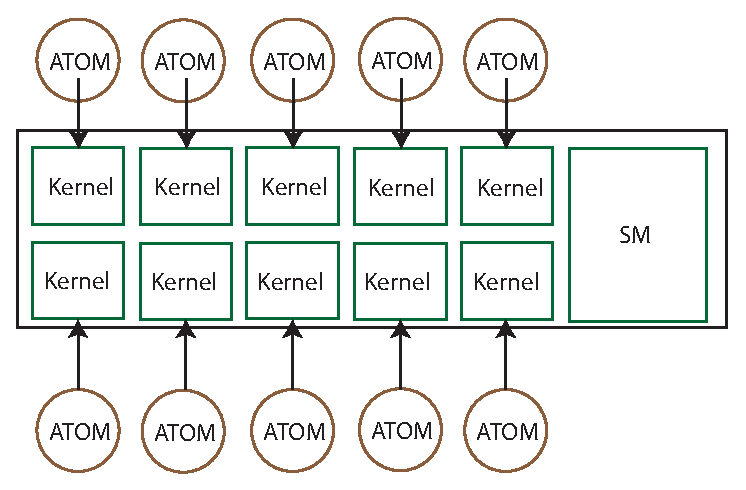
\includegraphics[width=0.5\columnwidth]{images/kernelatom.eps}}
\caption{ Example of atom mapping with kernels}
 \label{fg:kernelatom}


\end{figure}
%%%%%%%%%%%%%%%%%%%%%%%%%%%%%%%%%%%
%%%%%%%%%%%%%%%%%%%%%%%%%%%%%%%%%%%

\subsection{Contribution and roadmap of the paper} 
The proposed improved version of push-based system for molecular simulation data analysis, we believe, gives an opportunity for scientists to run their analysis even faster now. Taking an advantage of GPU devices nature and incorporating parallelism and streaming for different types of queries, we have come up with a good speed up over sequential processing, which already had a good speed up in terms of performance in comparison with original pull-based approach. Since in this paper we don't expect certain form of data, we have come up with a tool that generates mock data for any number of atoms and frames, which can be used for performance tests that were done consequently, too. This mock data has exactly the same information that would come with Gromacs simulation files, and it has exactly the same format as in the previous paper \cite{mainPaper} right before loading it to memory. This improved version has been developed on Amazon Elastic GPU \cite{amazonGPU} nodes that consequently can be replicated and scaled up becoming more of a streaming distributed processing engine (which can be very effective on costs, since it is always easy to scale them up, shut them down and spin them back up), as well as on a simple desktop computer with a GPU device.
In general, major contribution of this paper is the framework of push-based system with an incorporated parallelism based on CUDA programming language. Besides it, there was developed a tool which generates mockup data of the same format as of the real MS simulations and represent a python script with arguments given as number of frames and atoms.

The structure of the framework which will be described later is developed in such a way that one can easily add new queries based on their complexity or modify existing ones adding appropriate selections and filters.


%%%%%%%%%%%%%%%%%%%%%%%%%%%%%%%%%%%%%%%%%%%%%%%%%%%%%%%%%%%%%%%%%%%%%%%%%%%%%%%

\vspace{3mm}
\section{Related Work}\label{sc:relatedwork}
\vspace{3mm}

Push-based system for MS data analysis is primarily proposing an idea of pushing chunks of data through a network of queries. Essentially, this has also been proposed, as mentioned already, by other frameworks \cite{DataPath,Volcano,Qpipe}. In other words, the major point is to use common data loaded into memory for execution of concurrent queries, which is supposed to eliminate I/O overhead predominantly. The architecture and explanation of DSMS (Data Stream Management System) versus DBMS is well explained in one of the lectures of Morgan and Claypool \cite{DataStreamManagement}. It is very important to capture the differences and specialties of DSMS in network architecture, stream models and windows, scheduling, load balancing, approximation, data expiration, etc, because of the fact that data flow design is the key that required all of those changes to common designs.

Since dealing with data is very delicate in this kind of engines, there are couple of features and requirements that this architecture is applicable to, in order to avoid inappropriate understanding or application of this approach in systems that were covered in the lectures\cite{DataStreamManagement}. The data is volatile and not persistent anymore because of obvious sizes of data.  Since we are pulling the data as little times as possible taking into consideration that MS data is only appended and not modified, the access is sequential rather than random. There are concepts of framing and windowing, and memory is limited in streaming engine, while in DBMS secondary storage is considered to be unlimited. Obviously, because of all of these features or requirements to data, the streaming engine frameworks have some limitations like going back into the history of data, since it is volatile. In fact, this has also been tried by Borealis Streaming Engine \cite{borealis}. On top of the fact that it is a streaming engine, as it was built based on Medusa\cite{medusa} and Aurora\cite{aurora}, it proposes distributed processing at this point having some features to handle errors and look back in the history. In our case, it is primarily a single data source, since it is based on the simulation, though in the future the simulation software systems might introduce distributed computing, too. It is also important to mention such projects as PeriScope\cite{PeriScope}, SciDB\cite{SciDB}, and other\cite{SDSS_SIGMOD02,QBISM_ICDE94}, since they target scientific data, which is a lot more different, than usual industry customer oriented data.

This version of Push-based System of MS data analysis is primarily about taking an advantage of GPU processing of the data. Hadoop is a well-known and well-used framework by many companies nowadays\cite{hadoop}. Its purpose is an ability to store and serve large scale data across clusters in a timely fashion. Since usage of GPU of massive data (not only related to graphics processing) is a relatively new concept, there is also an improved version of Hadoop MapReduce Framework with GPU\cite{hadoopgpu}. Having an ability to scale it up in a distributed computing environment is probably one of the best approaches, but again it might be a bigger overhead in terms of costs, since keeping all nodes up and still being able to solve specific problem sets with hardware stack of a lower capacity raise a will to explore more. Having a specific software for simulation like Gromacs, apparently there is also a possibility of taking an advantage of GPUs. For example, Gromacs allows to optimize simulation and query tools by adding configurations based on GPU device located on the processing computer. Unfortunately, even with this feature, Gromacs doesn't follow push-based approach which means that improvement with GPU with pull data per query makes it negligible.

Gromacs generate output files with physical properties description for each atom in each frame. Modern CPUs do great job in terms of caching and computing, but obviously in this particular problem massive monolithic computation is needed, thus, GPU devices are perfect candidates for such a problem following SIMD type of computation. To be more exact, for example, a single kernel in a GPU device could be dedicated to a single atom (this relationship might change depending on the query, but this is to understand the scale and relationship of multiprocessors), and since we have scientific data of MS, the data is appended, which means that we will only move forward and not take an advantage of caching on chunks high level (though we might take an advantage of GPU caching features particularly in processing phase) having multiple workloads per chunk. Just to make it more clear, workloads in this particular case represent transactions based on number of clients. For example, if we were to serve it all in a streaming fashion, 100 clients might demand concurrent queries with different slight selection properties and expect their results, each workload might be dedicated to each client if not aggregated. Thus, the performance of GPU is certainly increasing based on workload too, which might benefit considerably.

%%%%%%%%%%%%%%%%%%%%%%%%%%%%%%%%%%%%%%%%%%%%%%%%%%%%%%%%%%%%%%%%%%%%%%%%%%%%%%%

\vspace{3mm}
\section{Network of Queries}\label{sc:querynetwork}
\vspace{3mm}

Having generated big amount of data in large files, now scientists need to get useful information out of it by means of analysis utilities. Often times, the queries that need to be run over the data look like selection and some kind of accumulation, if it is not more complicated. To be more exact, in this section we will try to summarize common set of queries we will be improving. 

In previous work, there has already been developed a network of queries widely used by scientists for MS systems. In Table~\ref{tb:queries} you may observe the common set of queries that has been developed. Basically, these are the queries that need to be improved with our new approach of parallelism. Just to mention, $n$, $r_i$, $m_i$, $c_i$ and $q_i$ denote number of particles, coordinates (vector form), mass, charge, and number of electrons of a particle $i$.

\begin{table}[h]
\resizebox{\columnwidth}{!}{\begin{minipage}{\columnwidth}
\renewcommand*{\arraystretch}{1.5}
\tabcolsep=0.12cm
\begin{tabular}{|c| c|}
\hline %inserts horizontal line
Function Name & Equation/Description \\[0.5ex] \hline
Moment of Inertia & $\begin{array} {lcl} I & = & \sum\limits_{i=1}^n m_ir_i \end{array}$ \\[0.5ex]
\hline
Moment of Inertia on z axis & $\begin{array} {lcl} I_z & = & \sum\limits_{i=1}^n m_ir_{zi} \end{array}$ \\[0.5ex]
\hline
Sum of masses & $\begin{array} {lcl} M & = & \sum\limits_{i=1}^n m_i \end{array}$ \\[0.5ex]
\hline
Center of mass & $\begin{array} {lcl} CoM & = & \frac{I}{M} \end{array}$ \\[0.5ex]
\hline
Radius of Gyration & $\begin{array} {lcl} RG & = & \sqrt{\frac{I_z}{M}} \end{array}$ \\[0.5ex]
\hline
Dipole Moment& $\begin{array} {lcl} D & = & \sum\limits_{i=1}^n q_ir_i \end{array}$ \\[0.5ex]
\hline
Dipole Histogram & $\begin{array} {lcl} D_z & = & \sum\limits_{i=1}^n \frac{D}{z} \end{array}$ \\[0.5ex]
\hline
Electron Density & $\begin{array} {lcl} ED & = & \frac{\sum\limits_{i=1}^n (e_i-q_i)}{dz \cdot x \cdot y} \end{array}$ \\[0.5ex]
\hline
Heat Capacity & $\begin{array} {lcl} HC & = & \frac{3000 \cdot \sqrt{T} \cdot boltz}{2 \cdot \sqrt{T}-n \cdot df \cdot VarT} \end{array}$ \\[0.5ex]
\hline
Isothermal Compressibility & $\begin{array} {lcl} I & = & \frac{VarV}{V_{avg} \cdot boltz \cdot T \cdot PresFac} \end{array}$ \\[0.5ex]
\hline
Mean Square Displacement& $\begin{array} {lcl} msd & = & \langle (r_{t+\Delta_t}-r_t)^2 \rangle \end{array}$ \\[0.5ex]
\hline
Diffusion Constant & $\begin{array} {lcl} D_t & = & \frac{6 \cdot msd(t)}{t} \end{array}$ \\[0.5ex]
\hline Velocity Autocorrelation & $\begin{array} {lcl} V_{acor} & =&
\langle (V_{t+\Delta_t}\cdot V_t) \rangle \end{array}$ \\[0.5ex]
\hline
Force Autocorrelation & $\begin{array} {lcl} F_{acor} & = & \langle (F_{t+\Delta_t} \cdot F_t) \rangle \end{array}$ \\[0.5ex]
\hline
Density Function & Histogram of atom counts \\[0.5ex]
\hline
SDH & Histogram of all distances \\[0.5ex]
\hline
RDF & $\begin{array} {lcl} rdf(r) & = & \frac{SDH(r)}{4 \cdot \pi \cdot r^2 \cdot \sigma_r \cdot \rho} \end{array}$ \\[0.5ex]
\hline
\end{tabular}
\caption[Table caption text]{Popular analytical queries in MS\cite{mainPaper} }
\label{tb:queries}
\end{minipage} }
\end{table}

In general, with the given queries we have divided them into two categories: one body functions and multiple body functions. The first ones apparently have linear complexity of $O(n)$, while the other ones have bigger complexity. 

\emph{\textbf{One body functions}} such as sum of masses, center of mass, or simple counting with selection  are of a complexity $O(n)$, thus, in order to get the results for them going through every atom (essentially over the entire data) only once is enough, and taking into consideration the fact that we are going with push-based system, it is done at the same time for all of them. 

\emph{\textbf{Multiple body functions}} such as SDH and RDF (Spacial Distance Histogram and Radial Distribution function) require computation of distances pairwise across all the particles. This is generally combination of two across N data: 	$C\binom{N}{2}$. These are the most expensive queries, thus, it is important to focus on their implementation taking advantage of GPU nature and its processing power. SDH is a very expensive computation, and we have used some of the existing work of ours\cite{sdhgpu} to incorporate in this design.

The might be some dependencies and preliminary computation possibilities. For example, some queries need total mass, and we could compute it before we push it further, but this can be easily done by user based on the complexity and dependency. It is explained in more details in further sections.


\vspace{3mm}
\section{The system design}\label{sc:system}
\vspace{3mm}

The proposed design has a pretty straightforward structure which is going to be explained in this section. Shortly, the system starts with original input files (or data) and gets consumed in a sequential manner by simple disk IO framework into random access memory by chunks, then, chunk gets uploaded to GPU device and processed. At some point, the results that need to be shown to the user are transported from global memory of GPU (where they initially get accumulated) to the main memory, and then might get written as well to an output file. General data flow map is represented in Figure  \ref{fg:data-flow}.

\begin{figure}
 \centerline{ 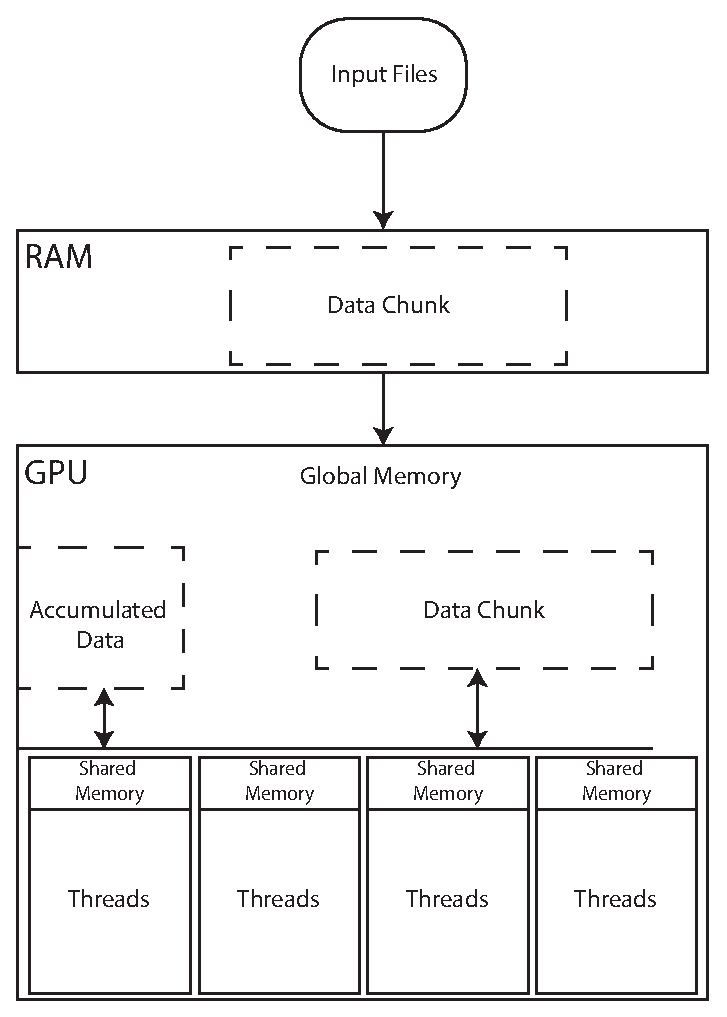
\includegraphics[width=0.65\columnwidth]{images/memory-organization.eps} }
 \caption{Data flow in the improved design of push-based system for MS analysis}
 \label{fg:data-flow}
\end{figure}

\subsection{Data input}
Since the size of the data in the problem is huge, organization of the data flow is crucial. As mentioned before, original data is retrieved from simulation software output files and in our case it is Gromacs Software's trajectory files\footnote{The file types, their structure, and their decompression has been well explained in the previous paper in section "Data orgranization in main memory"}. For a simulation, there can be several files of different format and usually they are also compressed without any loss of information. Tool for decompressing those files to a flat format for each frame and atom has been developed in the previous work\cite{mainPaper}. 

In order to experiment with different input cases, the input files have been generated with a tool that we have built in Python language. Thus, we are able to generate mock data files with any number of frames and atoms, and the values are random and can be adjusted with needs of the experiment (for example, for cases when we want to analyze bucket widths in a limited space, the coordinates are generated in range of $0 - 1$, etc.). As it has already been mentioned earlier, we don't expect the data to be distributed with a certain behavior, the importance of having this kind of tool to generate mock data is having a variety of random data sets that could reveal any issues related to values provided to the program, on top of that, having the actual file written and then being read has been a part of the experiments to have more realistic use case. In the future, the same script for generating the mock data could be used for regression and performance tests in a distributed implementation of this design as a single source.

\subsection{Data flow architecture}

MS data roughly can be represented as a list of atoms with physical properties aggregated as frames. Thus, we consider a single frame as a chunk which will be loaded into the memory\footnote{Memory in this design might be interpreted differently, since we have a separate device memory on GPUs, but it will be explained better later} and pushed through our network of query. In this case, it is very convenient, because there are almost no dependencies between frames, rather than list of atoms in the same frame, which potentially again could create additional disk I/O overhead.

Having defined the chunk, we load it from flat format file to RAM. A single atom data structure has all the attributes such as charge, mass, velocity, type of atom, coordinates, and so on. In other words, we have an array of atoms, and most of the attributes (in case of data structure, it is a class field), are simply primitive floats or doubles depending on precision requirements. Next, the same chunk of data with the same structure is loaded onto GPU global memory. GPU devices, in general, have about 4-5 types of memory, and global memory is the biggest and slowest. Consequently, depending on algorithm or query we load parts of data chunk to another types of memory called shared memory. It depends on the actual query, because the same part of chunk can be loaded and unloaded in regards with shared memory several times, especially with SDH.


\subsection{Network of queries organization}

Since we assume that our framework should be easily used by a scientist doing MS analysis, it is important to keep queries module as a separate piece of code to make it easily extendable. In order to understand how queries module is organized and the reason for it, we need to understand how CUDA and GPU work.

\emph{\textbf{GPU execution}}. From hardware standpoint, it is important to understand that every GPU device consists of SM (streaming multiprocessors), and each SM has thousands of registers, which can be partitioned among execution threads. Having this in mind, since this is a pure parallel processing power, the goal is to increase hardware throughput and keep highest utilization to exploit every register given. CUDA is an amazing tool that tries to help developers map this hardware capabilities with the actual application layer. In CUDA we have grids, blocks, and threads, where grid is 3 dimensional unit where each cell is a block, and the same relationship applies between blocks and threads\footnote{This explanation doesn't include memory setup in GPU devices, but it is covered in further sections}. Originally, this mapping was perfect for solving image processing problems or other graphics computation, since dimensions and such division (e.g. by pixels to threads) is very inherent. As a language feature, in CUDA we have to define such a function called 'kernel' function. Essentially, it is the function where we are supposed to map every execution thread with data and perform the actual execution, this approach is widely known as SIMD\footnote{SIMD - Single Instruction Multiple Data}. As a convenience we have separated one-body functions with multiple-body functions into separate kernels.

\emph{\textbf{One-body queries kernel}}.
Commonly used CUDA array reduction\cite{gpureduction} makes the implementation of all the one-body queries obvious. Figure \ref{fg:reduction} nicely represents general idea of the data mapping, where each cell of the vector can be associated with a thread of execution in the kernel. Having an array of atom data structures, we reduce the array accumulating all the needed data from each atom's attributes. We don't expect much performance improvement from coalesced memory access, since the data structure for atom can eliminate any gain of coalesced memory access, though for specific types of queries it could be possible to aggregate certain attributes into merged arrays and take an advantage of it. In this case, the solution should be simple in order to keep it easily extendable for other simple one-body queries for a scientist to program. We fetch all the atoms from GPU global memory, since we use references to atoms once. In this case, allocating shared memory and copying it over would complicate the implementation and possibly create additional overhead for one time reference usage. Finally, memory transportation and data consumption are implemented for user, thus, he only needs to extend the queries module which consequently can be turned into plugins model.

\emph{\textbf{Two-body queries kernel}}.
SDH (or RDF) is the algorithm that requires special treatment in our design. The point, as mentioned earlier, is that this function requires more than one iteration of the given set of atoms, but rather all combinations of pairs in a given frame, thus, it is not linear complexity. An implementation of this type of query might be very non-intuitive because of the nature of GPUs. Another issue is that since to take an advantage on this type of computation, before writing an implementation for it, a user must have a good understanding of GPU architecture which makes the system less user-friendly. At this point, it is more important to achieve good performance improvement results and then take care of ease of system extensions. As we already mentioned, GPU threads execute in parallel and consume certain amount of work followed by best try of all hardware capacities utilization, but, unfortunately, it is also important to take care of equal workload for every thread independently, so, that utilization is kept high. For this reason, we've come up with a solution that should increase performance of the computation which will be described later.

\begin{figure}
 \centerline{ 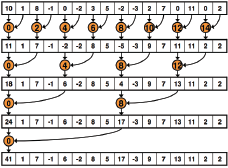
\includegraphics[width=0.65\columnwidth]{images/reduction} }
 \caption{Array reduction example\cite{gpureduction}}
 \label{fg:reduction}
\end{figure}

\begin{figure}
 \centerline{ 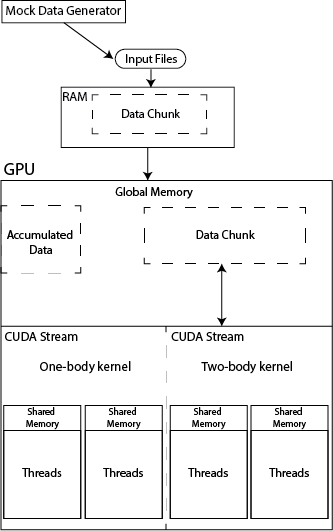
\includegraphics[width=0.65\columnwidth]{images/overallarchitecture} }
 \caption{Overall system architecture}
 \label{fg:overallarchitecture}
\end{figure}


\emph{\textbf{Architecture overview.}}
This section is to emphasize general architecture of the system and summarize the work flow as well as the data flow. In total, we have flat files with ready flat values for each atom aggregated in frames coming into the program as data input using common disk I/O framework of an operating system. Then, once we have loaded a frame (which is considered to be a chunk of the entire data set) onto RAM of our machine, we copy over the entire frame onto the GPU device global memory. It is important that, at this point, we never write any values to simulation files or any other data related to simulation, thus, we don't have to care about any synchronization of incoming data. After this, we have two predefined kernel functions (which were explained before), where first kernel stands for one-body queries, and the second one is for two-body query SDH. Just for architecture clearance and possible future improvements, two kernels are executed in two different streams\footnote{In CUDA stream is another abstract layer of organizing execution threads. They are not guaranteed to be executed at the same time or after each other, GPU scheduling architecture is completely different from CPU having a warp to be single scheduling unit at maximum of 32 threads at a time} (You can see them on Figure\ref{fg:overallarchitecture}). In each kernel we apply certain heuristics to improve memory access using such architecture features of GPU as shared memory and blocking of kernel threads.


\emph{\textbf{GPU grid and block sizes.}} As it has already been mentioned, utilization of hardware on GPU device is important, because it is the key to performance improvement, and the higher utilization is, the bigger improvement is.
The approach we came up with is 1 execution thread per atom. For CUDA version 2.0 maximum number of threads per block is 1024. Blocks are 3 dimensional entities in a 3 dimensional grid. The less abstract unit is, the less overhead we have in communication between them, thus, we try to utilize smallest units more. For example, for 1000,000 atoms, we would allocate 1024 threads per block as a static hard coded value, since we usually have always more than 1024 atoms in simulations. One dimension of grid can take up to 64,000 blocks, thus, if N is bigger than $1024 * 64,000$, than the rest would be allocated to $grid.y$ and $grid.z$ respectively. We have not considered numbers bigger than GPU can allocate, which could be explored in future work. It is important to understand that even though there are abstract entities of grids and blocks, it is not real hardware capacities, but they can affect scheduling and performance consequently. Decision to go with atom to thread execution is because it is pretty convenient to keep high utilization of hardware and still not lose idea if we are about to incorporate more functions, which makes the system more user-friendly, though later on as a plugin we left some room to add data transformer between RAM and GPU global memory, because there are a lot of custom ways to aggregate data and take an advantage of coalesced memory access.

\begin{figure}
 \centerline{ 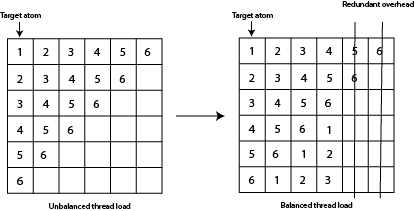
\includegraphics[width=1.0\columnwidth]{images/threadload} }
 \caption{SDH thread loading}
 \label{fg:threadload}
\end{figure}

%%%%%%%%%%%%%%%%%%%%%%%%%%%%%%%%%%%%%%%%%%%%%%%%%%%%%%%%%%%%%%%%%%%%%%%%%%%%%%%


\subsection{Computation work flow}

Once the data is loaded into global memory of GPU, we have two kernels for two types of queries setup for two different streams. Besides it, we allocate some memory in GPU global memory for results, too, and keep it as an object with fields to easily pull it back when it is ready, in our case all the data sizes are static before the kernels are executed, which follows nature of GPU devices. 
\subsubsection{One-body kernel} Every thread of execution in one-body query writes into shared memory, before accumulating the data into global memory result in order to avoid massive read and write blocking conflicts which will eliminate any kind of performance advantages. Once a block is finished, first thread of each block will accumulate data from shared memory into global synchronizing the results, every write operation to shared and global memories is atomic (e.g. generic CUDA function atomicAdd). We run the first stream with one-body queries and wait till it gets finished. The reason is that we expect certain behavior from shared memory from each of the streams, thus, just to make sure that they don't overlap, we run them separately. While the computation is running, there is a possibility to use a third stream to load another chunk of data, too. First stream and kernel execute simple vector reduction type of computation accumulating all the needed data and keep it in the GPU.
\subsubsection{Two-body kernel} Once the first kernel is finished we run the two-body kernel with its own stream. As it has already been mentioned, the biggest workload is in this kernel, because it has higher complexity. In this particular case it is $O(n^2)$. GPU streaming multiprocessors are very powerful for straightforward primitive independent calculations, and each core is much weaker than a moden CPU which has a whole bunch of L caches with some prediction behavior systems for code divergence. As you can see on Figure \ref{fg:threadload}, unbalanced thread load assumes for GPU kernel to check every time if the target atom can interact with other atom and if it has to wait till other threads finish their jobs. Thus, we had to come up with a strategy of making equally balanced thread jobs and distribute them among the threads leaving atom to thread mapping as is. 

For SDH we the following strategy

\begin{itemize}
\item[1.] Find current index (for target atom)
\item[2.] Find range of atoms it has to interact with in an equally loaded fashion
\item[3.] Load the range of atoms into shared memory
\item[4.] Iterate through the range of atoms from shared memory and atomically write the distances counts into buckets pre-allocated in share memory
\item[5.] Synchronize with other threads in the block (not in the entire grid)
\item[6.] If it is the first thread in block, add all bucket counts from shared memory into global memory
\end{itemize}


%%%%%%%%%%%%%%%%%%%%%%%%%%%%%%%%%%%%%%%%%%%%%%%%%%%%%%%%%%%%%%%%%%%%%%%%%%%%%%%

\section{Experimental results}\label{sc:experiments}

The system was implemented in C++ programming language and tested on
real molecular simulation data sets. The experiments were carried
out on an Apple MacPro machine with 8GB of physical memory and two
Quad-Core Intel Xeon 3GHz processors. The MacPro was running OS X
Mavericks $10.9.3$ operating system. We have compared the results
obtained by our system to those obtained by running the analysis
through GROMACS (v. $4.5.7$). Both systems were analyzing the same
data sets.

\emph{\textbf{Data sets.}} In our experiments, six data sets from
different simulations were used. All simulations were done on a
POPC~\footnote{POPC is a chemical compound composed of a
diacylglycerol and phospholipid. Its full name is
1-palmitoyl-2-oleoyl-sn-glycero-3-phosphocholine and it is one of
the most important lipids in bio-physical molecular simulation.}
lipid bilayer, but were all set to produce data of different sizes
(i.e., different number of particles in the simulation). Namely, we
have tested the system on simulations with $52,400$; $209,600$;
$838,400$; $2.5M$; $4.4M$; and $8.8M$ atoms. Also, since the
simulations were run separately, they produced six different MS
systems with distinct characteristics (distinct structure, atom's
positioning, etc.). From all of the generated data sets we have
randomly selected sets of $10$, $100$, and $1000$ consecutive frames
for the purpose of our experiments. This gave us $18$ different
datasets on which we tested our system.

\emph{\textbf{Query work load.}} Two types of query workload were
used: 1) one involving one-body queries only 2) one including
two-body queries (SDH and RDF) as well. The reason for this is that
GROMACS, the system we used to compare our system to, only has a
naive method of solving the RDF (SDH) problem (like almost all MS
analysis systems). In our system we have incorporated SDH (RDF)
algorithms that are far more superior to the naive method, and
comparing the systems like that would not have been fair (we
believe).

\emph{\textbf{One-body queries only.}} The following set of one-body
queries were included in the test workload: mean square displacement
(msd), radius of gyration, dipole moment, center of mass, velocity
autocorrelation, electron density, mass density, and charge density.
This set of queries were pointed to us, by a group in the physics
field with extensive MS background, as one of the most commonly used
in the field of collagen bilayer MS system analysis. A workload
group contains all $8$ queries executed on one of the $12$
selections, making $12$ groups. Such groups are executed on six
different size data sets, with $10$, $100$ and $1000$ frames. This
workload is then repeated $5$ more times, by executing each of the
queries in the groups $5$, $10$, $25$, $50$, and $100$ times,
essentially just magnifying the workload intensity. In total, we
have $12 x 6 x 3 x 6 = 1,296$ different workload setups to test the
system on. Fig.~\ref{fg:workload_set_up} shows the organization of
the workload setup.

%%%%%%%%%%%%%%%%%%%%%%%%%%%%%%%%%%%%%%%%%%%%%%%%%%%%%%%%%%%%%%%%%%%%%%%%%%%%%%%

\subsection{Benchmark}

Through extensive collaboration with a research group from the
Physics department at USF, we have come up with a benchmark that can
be used for testing the efficiency of an analysis system for
molecular simulations. The benchmark consist of three essential
parts: 1. Simulation data produced by an MS, 2. Queries that are to
be executed onto that data in order to produce some information of
interest, and 3.Benchmark parameters that control the size of the
benchmark.


\subsubsection{Benchmark Data}
The data used in the benchmark was real molecular simulation data,
produced through the GROMACS MS system. The initial, pre-simulation
data file consisted of $200$ POPC and $12000$ solvent molecules, or
$12200$ molecules in total. This type of system was used because it
is sufficiently diverse, containing enough distinct POPC and solvent
molecules (e.g., each POPC molecule includes approximately $52$
different atoms) and yet simple enough to be easily transformed into
another system of different size. By using the $genconf$ function in
GROMACS, we produced pre-simulation files of different sizes
(essentially by changing the system's size (box)). $Six$ different
sized pre-simulation files were created. A molecular simulation was
then run on these $6$ files, each producing an MS system of certain
size (volume/number of particles). All of the simulations were set
up to produce $1000$ frames (snapshots in time of the systems), each
frame containing the same number of particles as the base one. The
produced files contained: $52,400$; $209,600$; $838,400$; $2.5M$;
$4.4M$; and $8.8M$ atoms per frame. So, for example, the file with
$52,000$ atoms holds $52,000,000$ records in total ($1000$ frames,
each containing $52,000$ records). As mentioned earlier, this
simulation data comes mostly in binary formats and in trajectory
files having a lot of unneeded overhead. Therefore, it was
transformed to a data arrays files containing only crucial
information of the particles and the system. The size of the files
ranged from $135MB$ for $52,000$ atoms to $24GB$ for $8.8$ million
atoms (this is for data with $100$ frames).

%Fig.~\ref{fg:dataformat} represents the organization/structure of
%these files.

\subsubsection{Benchmark Queries}
The queries selected to be included in this benchmark were derived
through a thorough observation of the way an MS system is being
analyzed. They were found to be the base of the analysis of many MS
systems. In other words, no mater how small or big the analysis was,
these queries were included in that analysis. As mentioned earlier,
they are of two types: one-body (and algebraic) and two-boy (and
holistic). Table~\ref{tb:queries} shows these queries.


\subsubsection{Benchmark Parameters} There are several parameters
that can be used to control the overall size of the system. We divide the parameters into two groups:\\
Data size parameters:
\begin{itemize}
\item[-]Select different sized dataset
\item[-]Number of frames
\item[-]Data selection (within the selected dataset) onto which the queries are being executed
\end{itemize}
Workload size parameters:
\begin{itemize}
\item[-]Number of queries to be executed
\item[-]Number of times each query is executed
\end{itemize}
By changing these parameters, we can produce a versatile testing
benchmark for MS analysis systems.

%%%%%%%%%%%%%%%%%%%%%%%%%%%%%
\begin{comment}

\begin{figure}
 \centerline{ 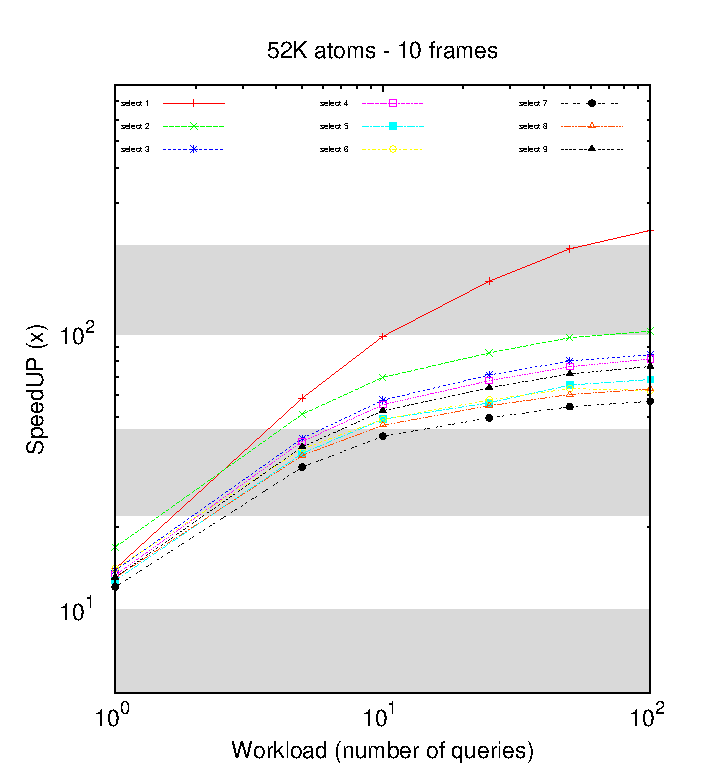
\includegraphics[width=columnwidth]{images/speedup10frames52K.eps} }
 \caption{Showing speedup for different workload}
 \label{fg:results2-10frames}
\end{figure}

\begin{figure}
 \centerline{ 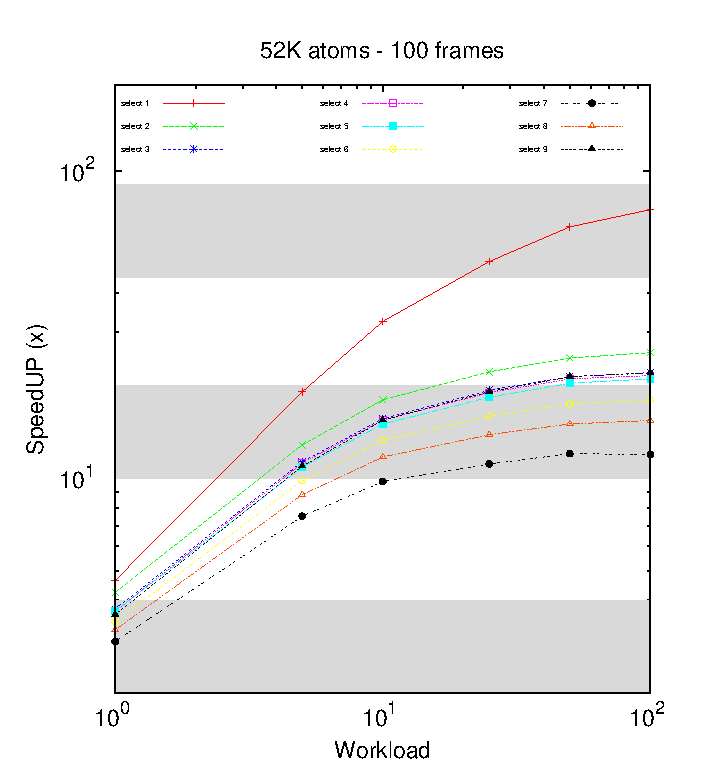
\includegraphics[width=columnwidth]{images/speedup100frames52K.eps} }
 \caption{Showing speedup for different workload}
 \label{fg:results2-100frames}
\end{figure}

\begin{figure}
 \centerline{ 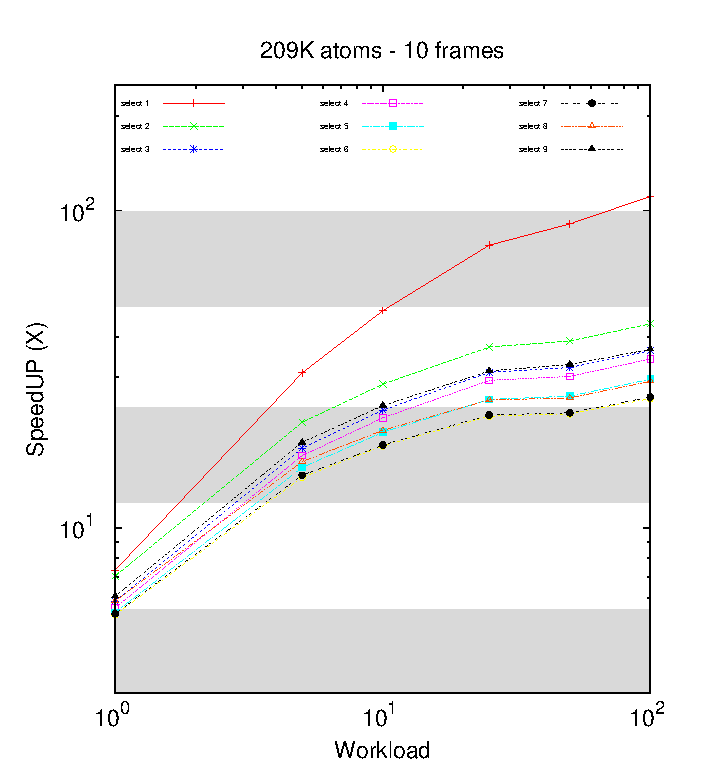
\includegraphics[width=columnwidth]{images/speedup10frames209K.eps} }
 \caption{Showing speedup for different workload}
 \label{fg:results3-10frames}
\end{figure}

\begin{figure}
 \centerline{ 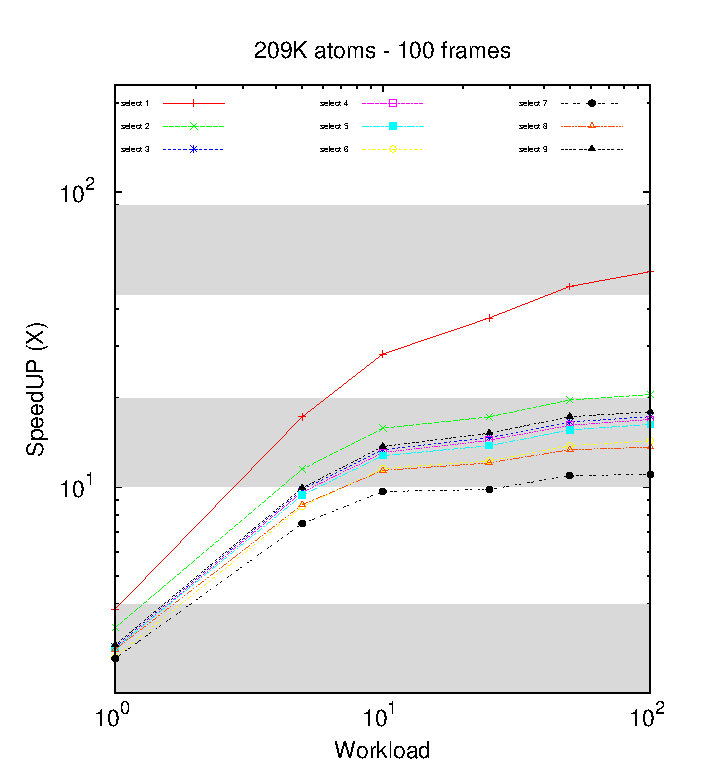
\includegraphics[width=columnwidth]{images/speedup100frames209K.eps} }
 \caption{Showing speedup for different workload}
 \label{fg:results3-100frames}
\end{figure}

\end{comment}
%%%%%%%%%%%%%%%%%%%%%%%%%%%%%%%%%%%%%5


%\begin{figure}
% \centerline{ 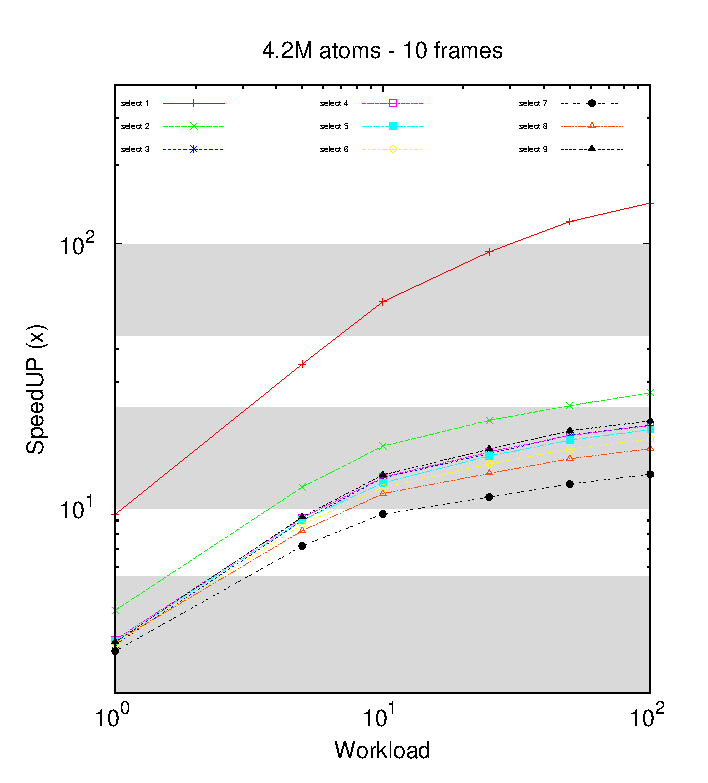
\includegraphics[width=.8\columnwidth]{images/speedup10frames4.2M.eps} }
% \caption{Showing speedup for different workload}
% \label{fg:results5-10frames}
%\end{figure}

\subsection{Results} We have run extensive experiments over all the
different setups of workload mentioned previously in this section.
However, in this paper we present only the workload setups of $4$
data size sets: $838,400$, $2.5M$, $4.2M$, and $8.8M$ atoms because
we believe they convey enough information about the efficiency of
our system compared to that of the Gromacs system. The running times
of our push-based system were compared to those of the Gromacs
system. The first set of figures, namely
Figures~\ref{fg:speedup838K-select-level}-\ref{fg:speedup8.8M-select-level},
represent the speedup that our system obtains over the Gromacs
system with various atoms selection levels. We define the selection
levels based on the number of comparisons we have to make in order
to extract the needed group(selection) of atoms. For example, if we
want to do analysis on all molecules containing oxygen, or hydrogen,
or carbon we would go over each molecule and compare its components
to the selection list. The bigger the selection list, the higher the
select level in our system. For better visualization, we note three
different selection levels: high (at least $10$ comparisons made),
medium (between $1$ and $10$ comparisons made), and low select level
(with one or less comparisons made). As seen in the figures, for
high selection level, the speedup is smaller compared to that
achieved in low select levels. The reason for this, we believe is in
that the amount of time our system spends extracting the atoms group
increases with the level of selection. Even though our system still
shows considerable speedup over Gromacs in high level selections, we
do believe there is room for improvement in our system and that is
our immediate future work we are planning on doing. These figures
also show the relation of the speedup to the workload intensity,
i.e., the higher the workload intensity the higher the speedup.

The connection between the workload intensity and the speedup is
better represented in the next set of figures,
Figures~\ref{fg:speedup838K}-\ref{fg:speedup8.8M}. They show the
speedup our system achieves over the Gromacs system on a varying
workload intensity. Each of those figures show the speedup with
different dataset sizes (e.g., $838,000$, $2,567,600$ atoms, etc.),
including $10$, $100$, and $1000$ data frames. The speedup is
calculated simply as a ratio between the running time of our system
on a certain set of workload and that of the Gromacs system on the
same workload. These figures show that the speedup over varying
workload intensity achieved by our system ranges anywhere from about
$10$ to $1000$ times, depending on the size of the dataset, number
of frames and the selection of the atoms.

Figure~\ref{fg:speedup-average-over-all-workload}, shows the speedup
our system achieves over all workload intensity (average workload
intensity) with varying dataset sizes. It is clear that, again our
system has better performance than the Gromacs system. The speedup
presented in this set of figures ranges anywhere from about $15$ to
$650$ times.


The last figure, Figure~\ref{fg:speedup-average-workload-select},
shows the speedup our system achieves over all workload intensity
and all select levels with varying dataset sizes. This figure, in a
way, summarizes the previous two sets of figures, bringing together
the workload and the different selections through the average. It is
clear that, again our system has better performance than the Gromacs
system. The speedup ranges anywhere from $50$ to $250$.

All four sets of figures show that such push-based design has clear
advantages over the pull-based type of design incorporated in the
Gromacs system.



\section{Conclusions and Future Work}\label{sc:conclusion}
The objective of our work is to design and implement improved data
analysis system that can be used in the field of molecular
simulation system's analysis. In this paper, we introduce the idea
for such system. We build our system on a push-based type design,
where data from data arrays is being pushed onto available queries
in the system. These queries are being executed on the pushed data
and produce intermediate / final result that would be used as part
of the data analysis. We are able to achieve an improvement over
existing, pull-based type designs because of the I/O overhead such
designs introduce when dealing with large volumes of scientific
data. Also, our queries are able to be executed on the same stream
of data, making it suitable solution for streaming circumstances. We
designed a benchmark that can be used to test data analysis systems.
This benchmark comprises of three parts: 1)benchmark data,
2)benchmark queries, and 3) benchmark parameters. We use this
benchmark to compare our system to one of the most frequently used
MS analysis systems, Gromacs. The efficiency and speedup achieved by
our system is supported by extensive experiments and their results.
The results show that our push-based design achieves up to about
$1000$ times speedup in comparison to a pull-based design, i.e.,
Gromacs.

One direction of our future work will be to further improve our
push-based design. Through the extensive experiments we have learned
that our design can be improved when the atom selection clause
involves many conditions. This improvement may be in the direction
of improving the algorithmic part, but it can also be in the
direction of improving the data presentation/organization we have
used in the system.\\

%%%%%%%%%%%%%%%%%%%%%%%%%%%%%%%%%%%%%%%%%%%%%%%%%%%%%%%%%%%%%%%%%%%%%%%%%%%%%%%


\noindent{\bf Acknowledgements:} The project described was supported
by an Award (R01GM086707) from the National Institute Of General
Medical Sciences (NIGMS) at the National Institutes of Health (NIH).
The authors would like to thank Anand Kumar who has contributed his
time and knowledge toward completion of the work.

%%%%%%%%%%%%%%%%%%%%%%%%%%%%%%%%%%%%%%%%%%%%%%%%%%%%%%%%%%%%%%%%%%%%%%%%%%%%%%%
%%%%%%%%%%%%%%%%%%%%%%%%%%%%%%%%%%%%%%%%%%%%%%%%%%%%%%%%%%%%%%%%%%%%%%%%%%%%%%%
%%%%%%%%%%%%%%%%%%%%%%%%%%%%%%%%%%%%%%%%%%%%%%%%%%%%%%%%%%%%%%%%%%%%%%%%%%%%%%%

\bibliographystyle{IEEEtran}
\bibliography{references.bib}

\clearpage

%%%%%%%%%%%%%%%%%%%%%%%%%%%%%%%%%%%%%%%%%%%%%%%%%%%%%%%%%%%%%%%%%%%%%%%%%%%%%%%
%%%%%%%%%%%%%%%%%%%%%%%%%%%%%%%%%%%%%%%%%%%%%%%%%%%%%%%%%%%%%%%%%%%%%%%%%%%%%%%

\appendices

%%%%%%%%%%%%%%%%%%%%%%%%%%%%%%%%%%%%%%%%%%%%%%%%%%%%%%%%%%%%%%%%%%%%%%%%%%%%%%%

\end{document}
